\documentclass[a4paper, 11pt]{article}

\usepackage[T2A]{fontenc}
\usepackage[utf8]{inputenc}
\usepackage[english, russian]{babel}
\usepackage{amsmath}
\usepackage{graphicx}
\usepackage{subcaption}
\usepackage{float}
\usepackage{tabularx}
\usepackage{amsmath,booktabs}
\usepackage{array}
\righthyphenmin=2
\usepackage[left=20mm, top=15mm, right=15mm, bottom=15mm, nohead, footskip=10mm]{geometry} % настройки полей документа
\usepackage{caption}
\DeclareCaptionLabelSeparator{dash}{ – }
\captionsetup{justification=centering,labelsep=dash}
\newcommand\tline[2]{$\underset{\text{#1}}{\text{\underline{\hspace{#2}}}}$}
\captionsetup[table]{justification=justified,singlelinecheck=false}
\begin{document}
	
		\begin{titlepage}
		\centering
		{\fontsize{12pt}{5cm}\selectfont \bfseries Министерство образования и науки Российской Федерации} \\ \vspace{0.5cm}
		{\fontsize{7pt}{5cm}\selectfont ФЕДЕРАЛЬНОЕ ГОСУДАРСТВЕННОЕ АВТОНОМНОЕ ОБРАЗОВАТЕЛЬНОЕ УЧРЕЖДЕНИЕ ВЫСШЕГО ПРОФЕССИОНАЛЬНОГО ОБРАЗОВАНИЯ} \\ 
		\vspace{1cm}
		{\fontsize{12pt}{5cm}\selectfont \bfseries САНКТ-ПЕТЕРБУРГСКИЙ УНИВЕРСИТЕТ ИНФОРМАЦИОННЫХ ТЕХНОЛОГИЙ, МЕХАНИКИ И ОПТИКИ} \\ \vspace{1.5cm}
		
		{\fontsize{14pt}{5cm}\selectfont Кафедра \hspace{1cm} \underline{Систем Управления и Информатики}  \hspace{1cm} Группа \underline{Р3340}} \\ 
		\vspace{2cm}
		
		{\fontsize{20pt}{5cm}\selectfont \bfseries Лабораторная работа №8} \\
		{\fontsize{20pt}{5cm}\selectfont \bfseries “Экспериментальное построение областей устойчивости линейной системы на плоскости двух параметров”} \\
		{\fontsize{14pt}{5cm}\selectfont Вариант - 02} \\
		\vspace{1.5cm}
		
		\flushleft
		
		{Выполнил \hspace{0.5cm} \tline{(фамилия, и.о.)}{10cm} (подпись)} \\
		\vspace{2cm}
		
		{Проверил \hspace{0.5cm} \tline{(фамилия, и.о.)}{10cm} (подпись)} \\
		\vspace{5cm}
		
		"\underline{\hspace{0.4cm}}"\hspace{0.1cm}\underline{\hspace{1.5cm}}\hspace{0.1cm}20\underline{\hspace{0.4cm}}г. \hspace{2cm} Санкт-Петербург, \hspace{2cm} 20\underline{\hspace{0.4cm}}г. \\ \vspace{1cm}
		
		Работа выполнена с оценкой \hspace{0.5cm} \underline{\hspace{10cm}} \\ 
		\vspace{1cm}
		Дата защиты "\underline{\hspace{0.4cm}}"\hspace{0.1cm}\underline{\hspace{1.5cm}}\hspace{0.1cm}20\underline{\hspace{0.4cm}}г.
		
	\end{titlepage}

	\section*{Цель работы}\hfill\par
	Ознакомление с экспериментальными методами построения областей устойчивости линейных динамических систем и изучение влияния на устойчивость системы ее параметров.
	\section*{Исходные данные}\hfill\par
	Необхожимо исследовать границу устойчивости системы при $g = 0$ , $y(0) = 1$ и $T_1=0.1$ изменяя $T_2$ от 0.1 до 10. \par
	Модель системы представлена на рисунке 1.
	\begin{figure}[h!]
		\center{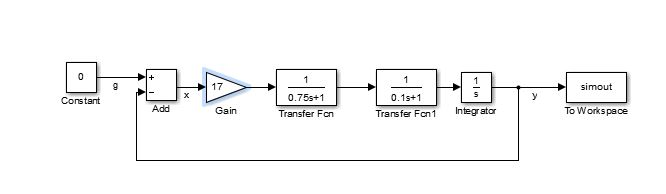
\includegraphics[width=1\linewidth]{1}}
		\caption{Модель исследуемой системы}
		\label{one}
	\end{figure}
	\newpage
	
	\begin{center}
		\section{Устойчивость системы}
	\end{center}

	На рисунках 2-4 показаны переходные характеристики системы при различных $K$. 
	\begin{figure}[h!]
		\center{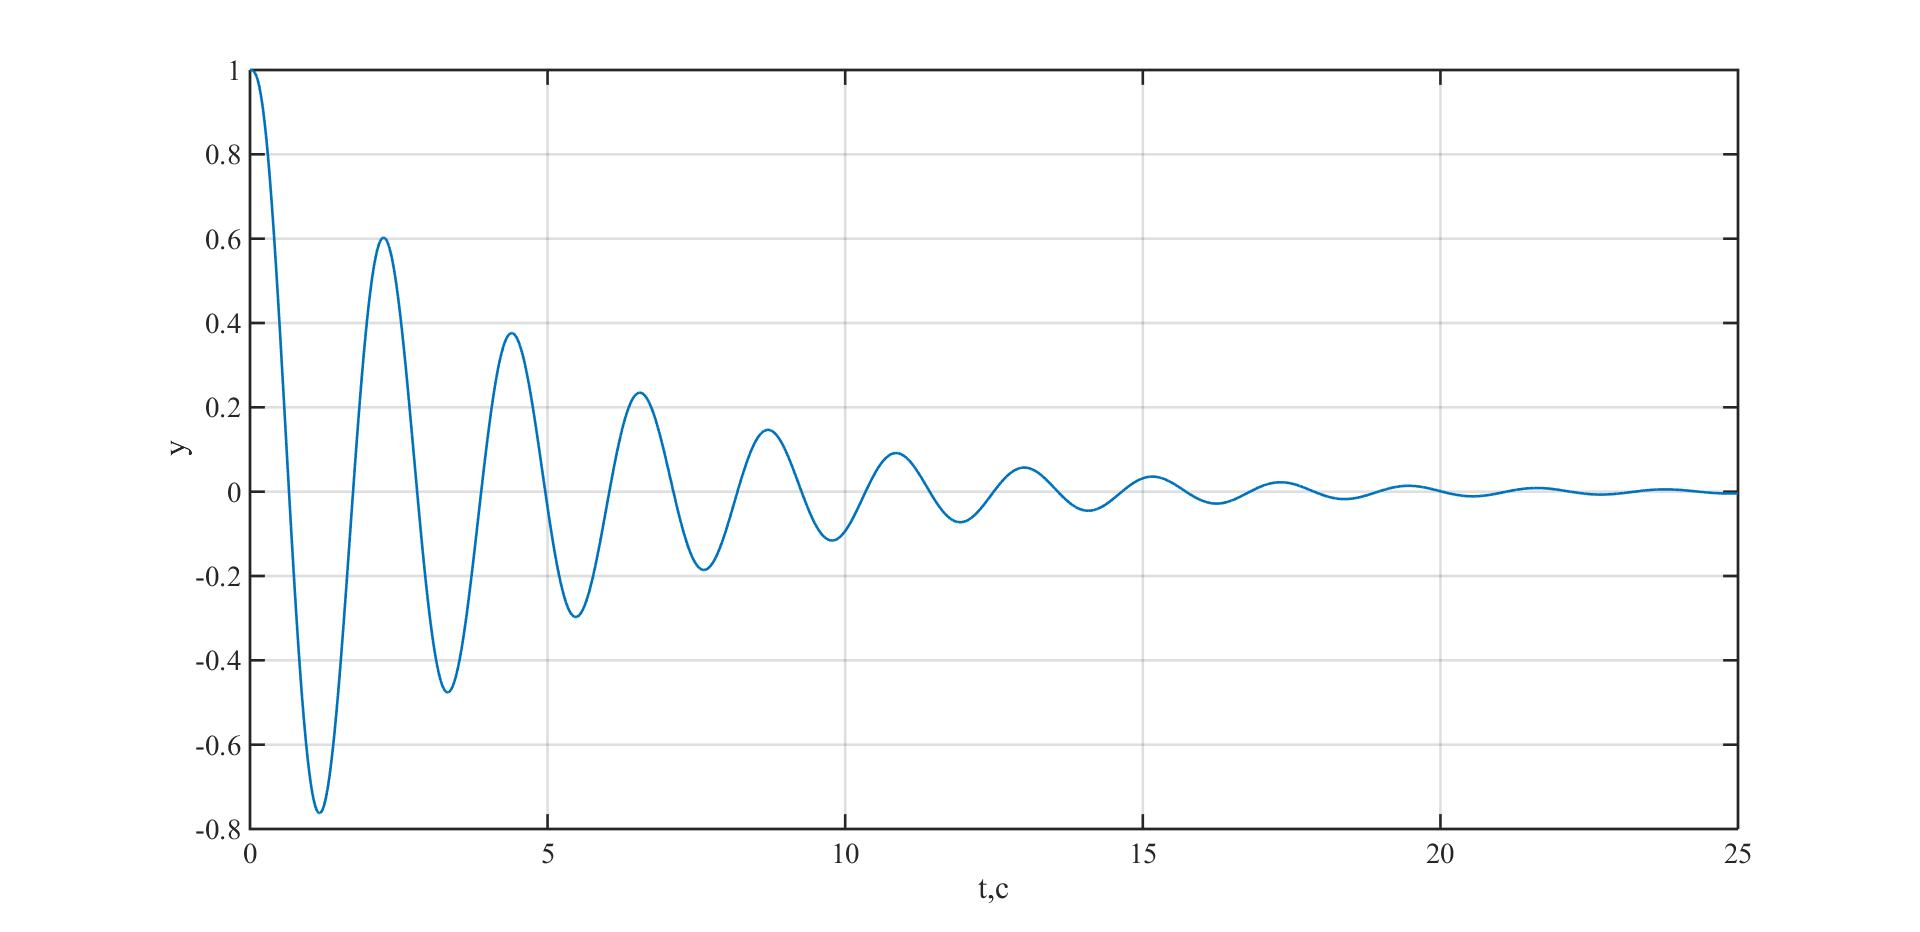
\includegraphics[width=1\linewidth]{1/1k7}}		\caption{Устойчивая система при K = 7}
		\label{2}
	\end{figure}
	\begin{figure}[h!]
		\center{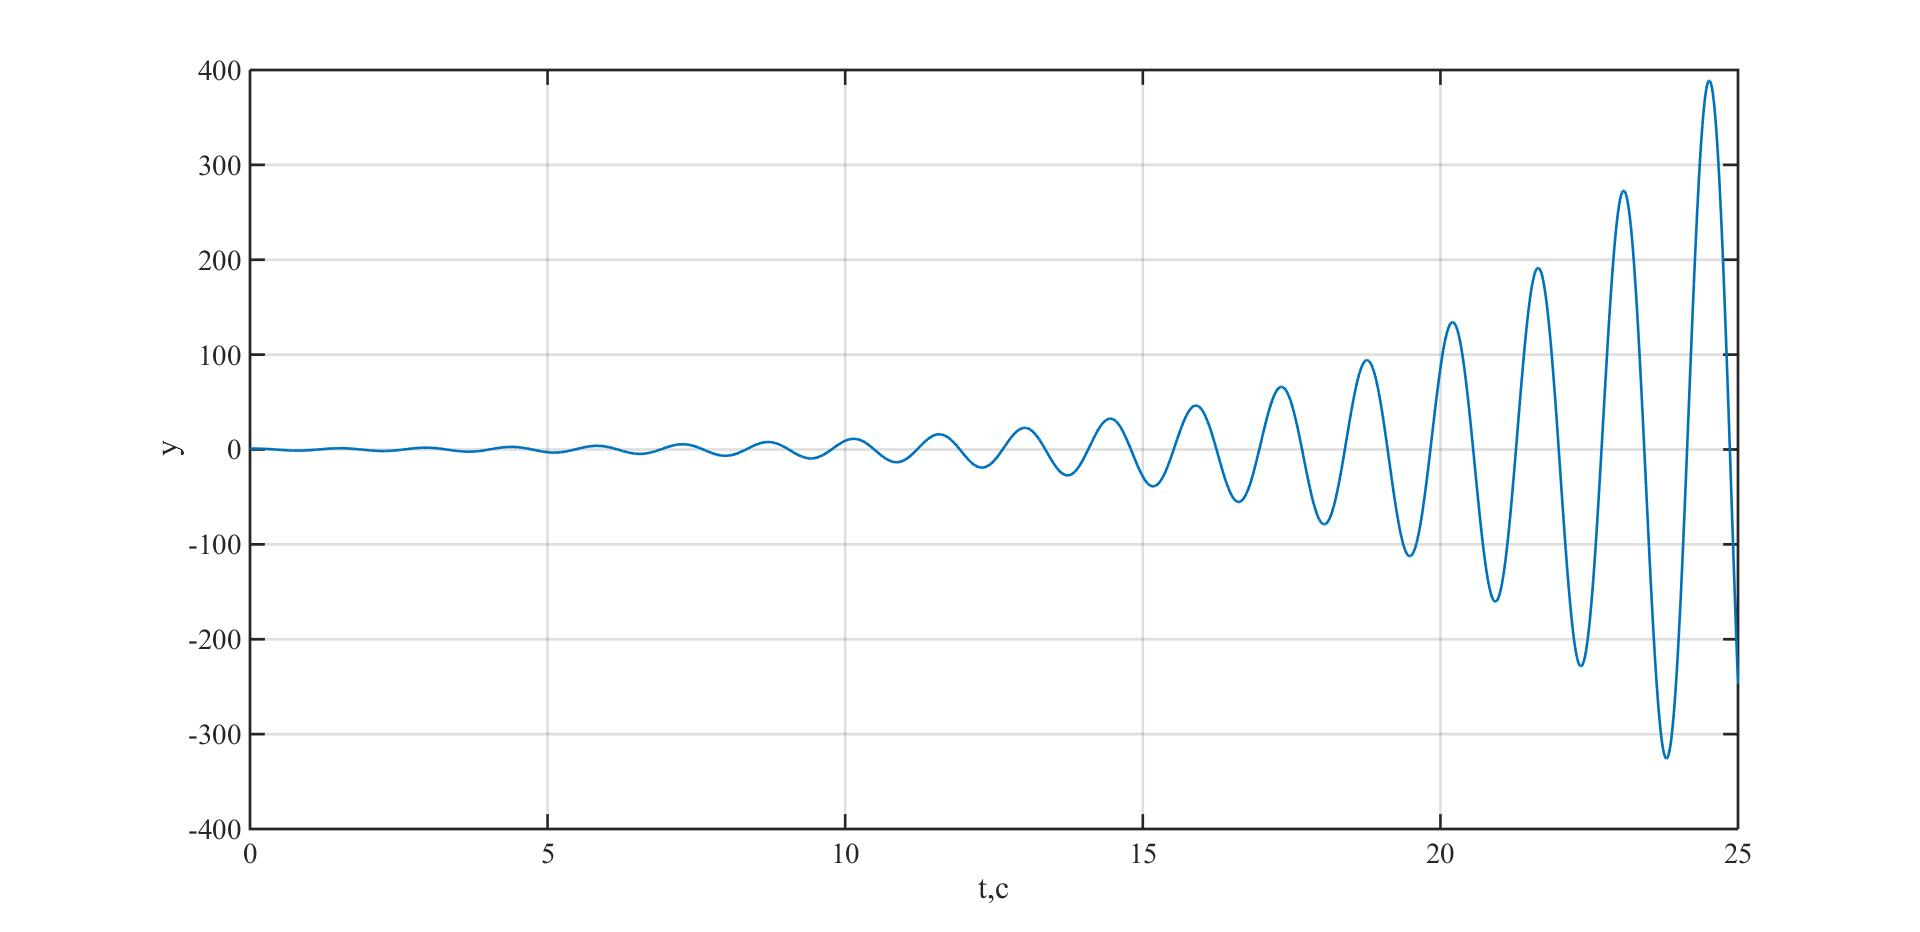
\includegraphics[width=1\linewidth]{1/1k17}}
		\caption{Не устойчивая система при К = 17}
		\label{3}
	\end{figure}

\newpage

	\begin{figure}[h!]
		\center{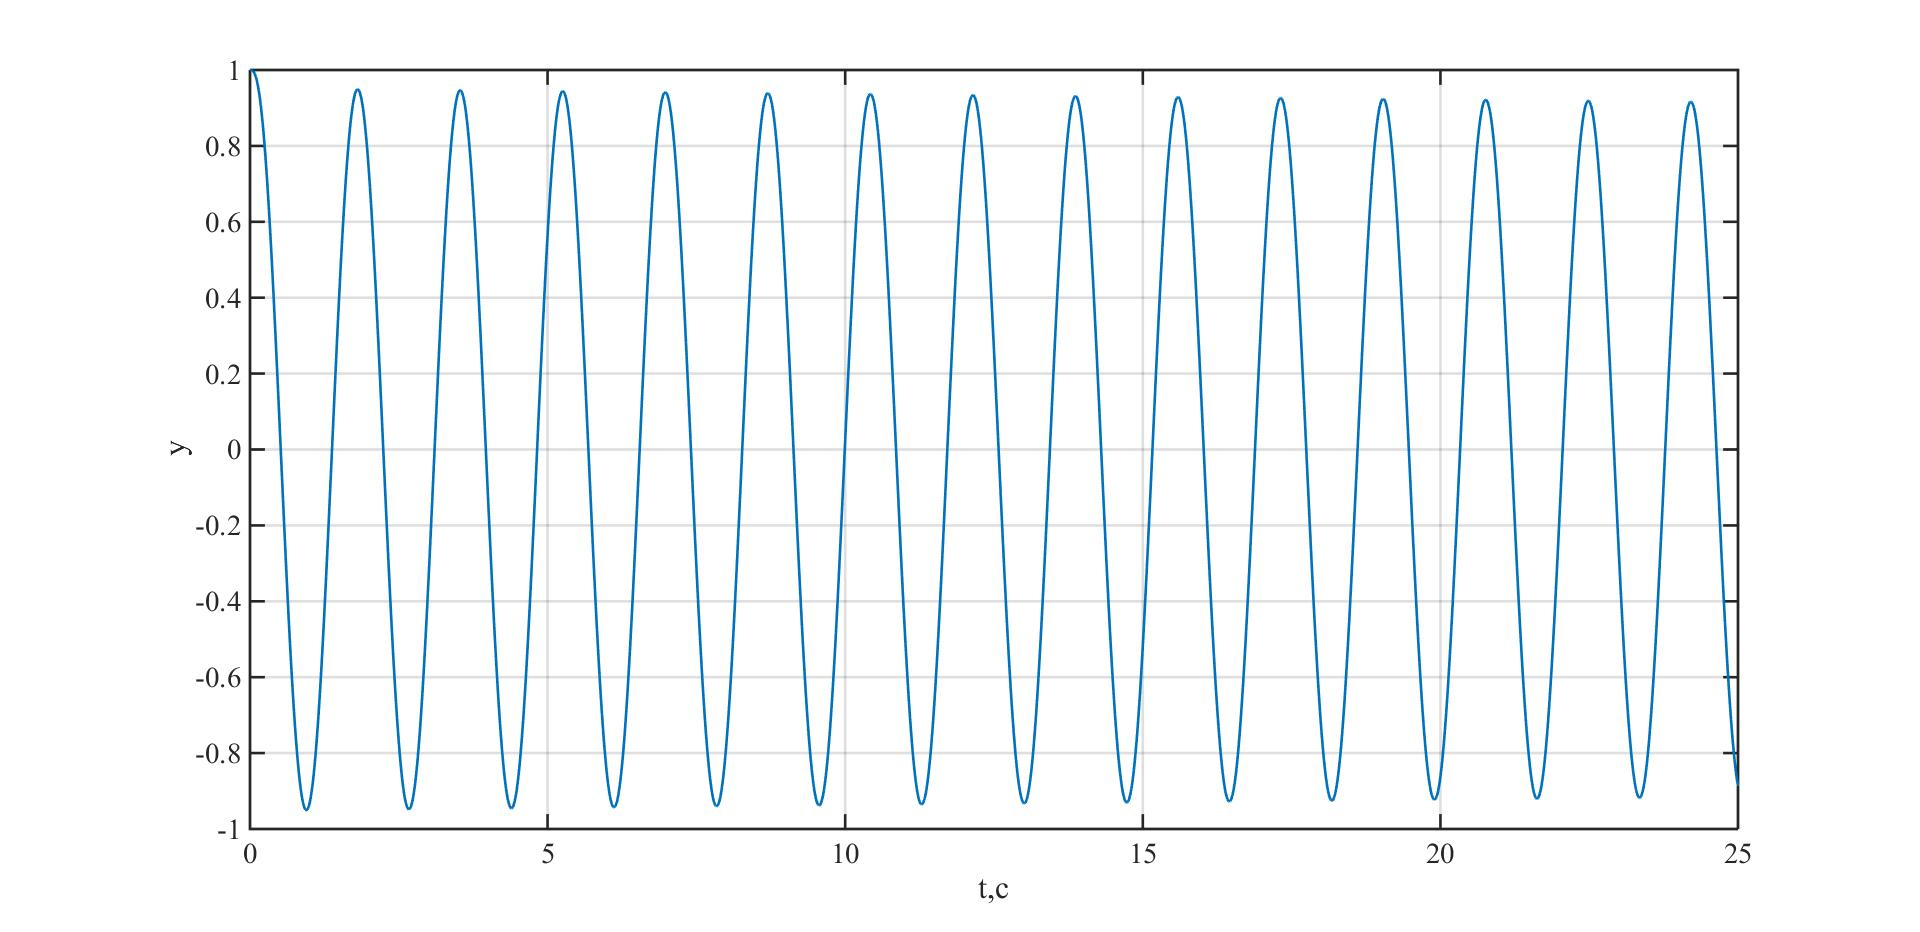
\includegraphics[width=1\linewidth]{1/1k11_3}}
		\caption{Система на границе устойчивости при К = 11.3}
		\label{11_3}
	\end{figure}
		
\newpage
%%%%%%%%%%%%%%%%%2%%%%%%%%%%%%%
	\begin{center}
		\section{Анализ устойчивости системы}
	\end{center}\hfill\par 
Из модели исследуемой системы можно вывести передаточную функцию:
	\begin{equation}
		W(s) = \frac{K}{T_1 T_2 s^3 + (T_1 + T_2)s^2 + s + K}
	\end{equation}
	
Для анализа устойчивости системы составим матрицу Гурвица.
	
	\begin{equation}
		G = \begin{bmatrix}
		T_1 + T_2 &  K & 0 \\
		T_1 T_2 & 1 & 0 \\
		0 & T_1 + T_2 & K
		\end{bmatrix}
	\end{equation}
	\hfill\par
Из этой матрицы можно вывести зависимость К от $T_1$ и $T_2$:
	\begin{equation}
		K=\frac{T_1+T_2}{T_1*T_2}
	\end{equation}
	
Произведем расчет границы устойчивости аналитически и сравним K.

\begin{table}[h]
	\caption{Зависимость коэффициента от ошибки}
	\begin{tabular}{|c|c|c|c|c|c|c|c|c|c|c|c|}
		\hline
		$T_2$ & 0.1 & 0.3 & 0.5 & 1 & 1.5 & 3 & 4.5 & 6 & 7.5 & 9 & 10\\
		\hline
		$K_r$ & 11.33 & 4.66 &3.33 & 2.33 & 2 & 1.66& 1.55 & 1.5& 1.46& 1.44& 1.43\\
		\hline
		$K_e$ & 11.3 & 4.6 & 3.3 & 2.3 & 2 & 1.6& 1.5 & 1.5 & 1.4& 1.4& 1.4\\
		\hline		    
	\end{tabular}	
	\label{tab:my_label}
\end{table}
	
На рисунке 5 построено отношение К расчетного, при увеличении $T_2$ и К экспериментального.

	\begin{figure}[h!]
		\center{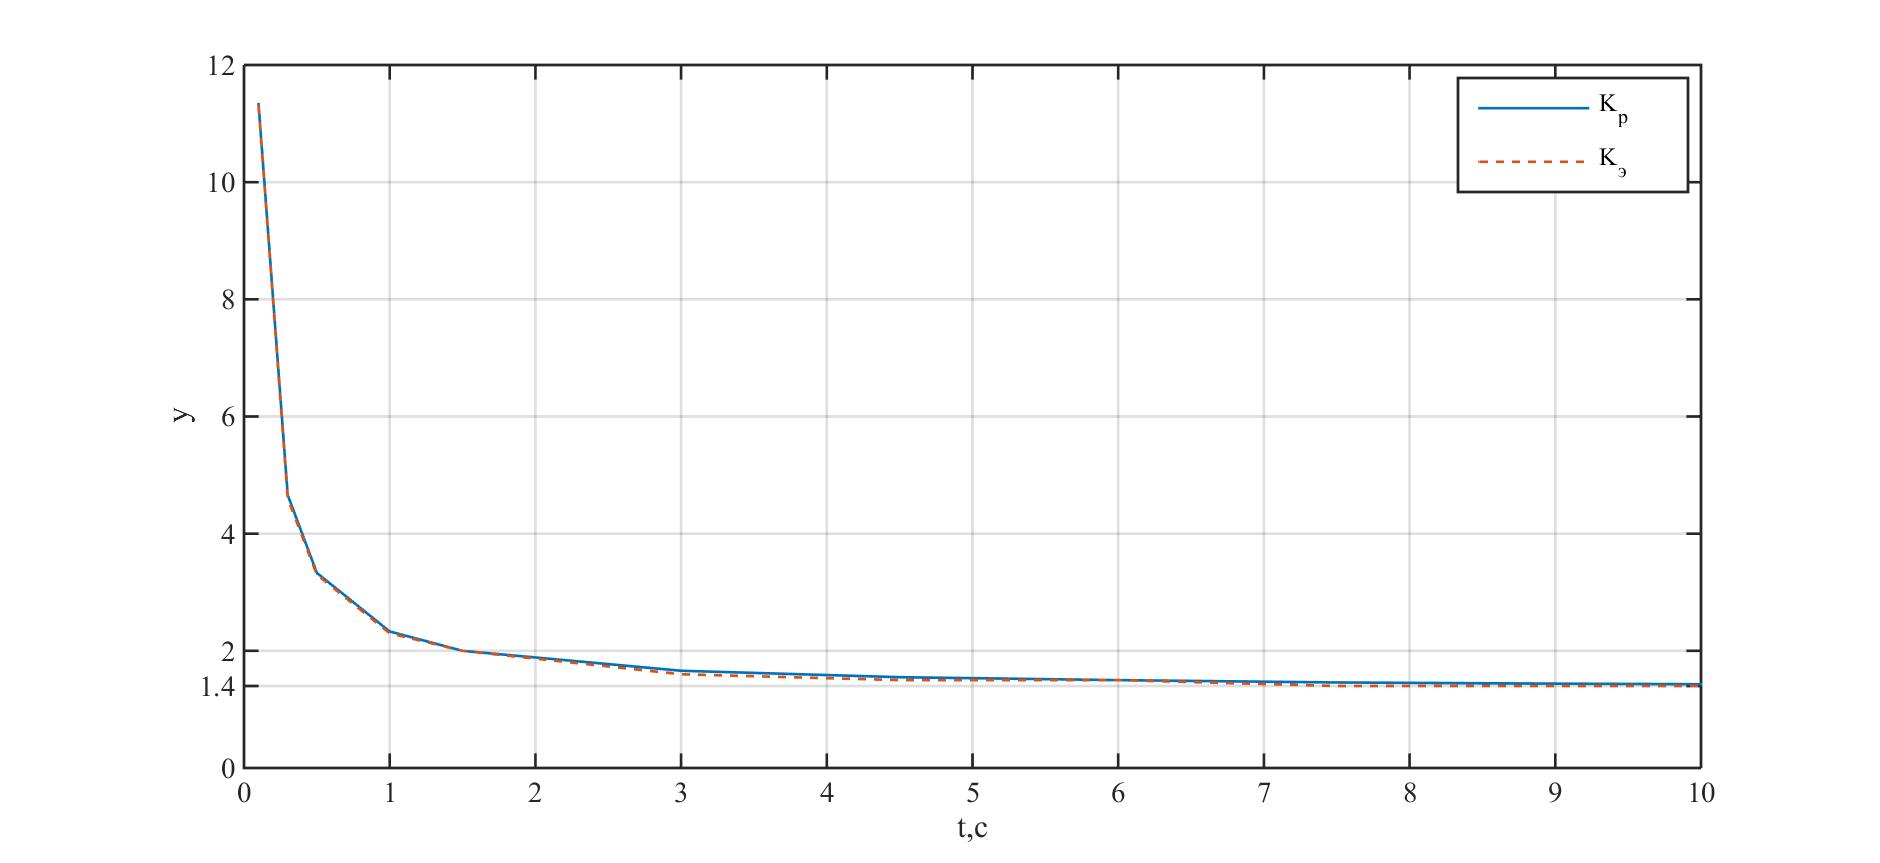
\includegraphics[width=1\linewidth]{final}}
		\caption{Граница устойчивости}
		\label{final}
	\end{figure}

\newpage 
	\begin{center}
		\section*{Вывод}
	\end{center}\hfill\par
В данной работе, изменяя параметры $K$ и $T_2$, а $T_1$ оставляя неизменным, с помощью математического моделирования и аналитических методов мы построили границы устойчивости системы исходя из условия Гурвица.

Данные, полученные при математическом моделировании и аналитическом методе совпали.





\end{document}